% !Mode:: "TeX:UTF-8"
%% 请使用 XeLaTeX 编译本文.
% \documentclass{WHUBachelor}% 选项 forprint: 交付打印时添加, 避免彩色链接字迹打印偏淡. 即使用下一行:
\documentclass[forprint]{software}
\usepackage{listings}
\usepackage{xcolor}
\usepackage{multirow}

\lstset{
	language=python,  %代码语言使用的是matlab
	frame=shadowbox, %把代码用带有阴影的框圈起来
	rulesepcolor=\color{red!20!green!20!blue!20},%代码块边框为淡青色
	keywordstyle=\color{blue!90}\bfseries, %代码关键字的颜色为蓝色,粗体
	commentstyle=\color{red!10!green!70}\textit,    % 设置代码注释的颜色
	showstringspaces=false,%不显示代码字符串中间的空格标记
	numbers=left, % 显示行号
	numberstyle=\tiny,    % 行号字体
	stringstyle=\ttfamily, % 代码字符串的特殊格式
	breaklines=true, %对过长的代码自动换行
	extendedchars=false,  %解决代码跨页时,章节标题,页眉等汉字不显示的问题
	%   escapebegin=\begin{CJK*},escapeend=\end{CJK*},      % 代码中出现中文必须加上,否则报错
	texcl=true}

\begin{document}

%%%%%%% 下面的内容, 据实填空.

\miji{ }                                      % 密级. 没有就空着.
\StudentNumber{202010311229} % 填写自己的学号

\title{应用软件开发课程设计\\在线文件编辑系统}
\Etitle{Online File Editor} % 英文题目
\author{孙思进}                            % 作者名字
\Eauthor{Sijin Sun}            %作者英文名
\Csupervisor{金世双\quad 老师}        %指导教师中文名、职称
\Esupervisor{Teacher Nan Yu}     %指导教师英文名、职称
\Cmajor{计算机科学与技术}                  % 专业中文名
\Emajor{Computer Science and Technology}% 专业英文名
\Cschoolname{信息工程学院}          % 学院名
\Eschoolname{College of Information Engineering} %学院英文名. 不确定的话, 请看一下自己学院的网页上是怎么写的. 别搞错了!
\date{二〇二二年五月}                    % 日期, 要注意和英文日期一致!!
\Edate{May, 2022}                       % 英文封面日期

%-----------------------------------------------------------------------------
\pdfbookmark[0]{封面}{title}         % 封面页加到 pdf 书签
\maketitle
\frontmatter
\pagenumbering{Roman}              % 正文之前的页码用大写罗马字母编号.
%-----------------------------------------------------------------------------
% !Mode:: "TeX:UTF-8"

%%%---- 郑重声明 (无需改动)------------------------------------%

\thispagestyle{empty}
\vspace*{20pt}
\begin{center}
	{\ziju{0.8}\pmb{\songti\zihao{2} 郑重声明}}
\end{center}
\par\vspace*{30pt}
\renewcommand{\baselinestretch}{2}
{\zihao{4}%
	
本人呈交的设计报告,是在指导老师的指导下,独立进行实验工作所取得的成果,
所有数据、图片资料真实可靠。 尽我所知,除文中已经注明引用的内容外,
本设计报告不包含他人享有著作权的内容。
对本设计报告做出贡献的其他个人和集体,
均已在文中以明确的方式标明。本设计报告的知识产权归属于培养单位。\\[2cm]
	
	\hspace*{1cm}本人签名: $\underline{\hspace{3.5cm}}$
	\hspace{2cm}日期: $\underline{\hspace{3.5cm}}$\hfill\par}
%------------------------------------------------------------------------------

\renewcommand{\baselinestretch}{1.5}  %下文的行距

\begin{cnabstract}
网络技术随着硬件的发展逐步提高,用户对高质量网络办公需求的情感越来越强,用户可以从中获取海量有用的信息,减少时间和资源的浪费。互联网在我国的政治、经济、生活上产生了非常大的影响,开发一款在线文本共享编辑系统可以有效地降低人们对办公位置的需求和限制,以此来实现居家办公的愿景。结合元宇宙、共享场景等概念,在线文本共享编辑成为了办公、学习、工作、国际交流的主流方式之一。本系统以python作为开发环境,结合MinIO和mysql分别作为文件管理系统和数据库管理系统,设计开发一款在线文档共享编辑系统。前端部分使用tkinter模块生成,后端模块通过flask框架接口生成。


\end{cnabstract}
\par
\vspace*{2em}

\cnkeywords{在线文档; 数据库; 服务器; flask }

\begin{enabstract}
With the gradual improvement of network technology with the development of hardware, users are more and more emotional about the demand for high-quality network office, and users can obtain a large amount of useful information from it, reducing the waste of time and resources. The Internet has had a great impact on our country's politics, economy and life. The development of an online text sharing editing system can effectively reduce people's needs and restrictions on office locations, so as to realize the vision of working from home. Combined with concepts such as metaverse and shared scenes, online text sharing and editing has become one of the mainstream ways of office, study, work, and international communication. This system uses python as the development environment, combined with MinIO and mysql as the file management system and database management system respectively, to design and develop an online document sharing and editing system. The front-end part is generated using the tkinter module, and the back-end module is generated through the flask framework interface.
	
	
\end{enabstract}
\par
\vspace*{2em}
\enkeywords{Online documents; database; server; flask}\\

\newpage
\cleardoublepage

\renewcommand{\baselinestretch}{1.5}
    % 加入摘要, 申明.
%==========================把目录加入到书签==============================%%%%%%
\pdfbookmark[0]{目录}{toc}
\tableofcontents
\mainmatter %% 以下是正文
%%%%%%%%%%%%%%%%%%%%%%%%%%%--------main matter-------%%%%%%%%%%%%%%%%%%%%%%%%%%%%%%%%%%%%
\chapter{引言}

\section{研究背景}

\section{背景}

随着5G通信技术在国内的迅速发展,加之疫情对实体线下接触的冲击,在线文档服务成为了办公、学习、工作、国际交流的第一选择,通过单台或者集群化的服务器(S端)连接全球各地的用户(S端)使用。在这个大背景下,在线文档企业异军突起,纷纷出现在人们的视野中。

办公需求的增加随着企业和行政的扩大而逐渐迫在眉睫,传统行政方式往往采用逐级递增的方法传递文档,使用繁琐的方式派发文件,处理效率极为低下。通过设计部署网络硬盘,是早期的在线文档的雏形。随之而来的,就是实现点对点单向修改文档的需求,最终,转向对多元化的网络文档管理。本文考虑到根据不同的企业对文档管理及通信的需要\upcite{r1},满足行政办公的在线文档编辑系统的设计和实现。

高速因特网通信技术给软件服务业的带来了新的发展空间,有效提高了软件服务业务经济能力、助力办公点对点、建设国家基建拓展业务的供求关系、加速发展重要软件的国产化和自主创新。在这种推动下,在线文档共享系统的应用将会为智慧办公、共享业务、中小企业的高质高量发展奠定坚实的基础,使互联网的使用成本逐步下降,从而拓宽更多企业的发展空间,让更多的用户体验到信息化时代的便捷性和优越性,为每一位用户实现需求差异化、需求定制化服务。本系统深入调查在线文本共享编辑系统在设计、应用的阻力和方向。

本设计研究了在线文本共享编辑系统的用户需求、功能需求、服务器部署、程序编写,深入调查在线文本共享编辑系统在设计、应用的阻力和方向,最终完成在线文本共享编辑系统的实现,创建一个基于基础功能、协同编辑、云服务化的需求,给使用者提供一个办公文档平台的体验。最终围绕在线文本共享编辑系统的主题进行研究,实现在线文本编辑、在线文本分享的功能,用户也可以上传自己的文本,共享给其他用户。

用户往往需要提交一些有关个人以及公司较为敏感的数据类型,首要任务是确保对文档数据的安全维护。目前来说,现有文件都是针对文档协同的过程进行加密,往往忽视了对文档储存的过程的保护。本设计采用了minio的文件管理服务器,提供一种纠错码的储存方式,既可以增加文档储存的安全性,又增加了文档防窃取的安全性。

考虑到本系统可能部署在网络上,我们需要对用户密码的储存进行加密,采用的方法是对密码文本取md5校验码,储存在数据库服务器。

系统的功能模块设计是否完整、合理, 决定了系统性能的优劣, 根据实际情况对系统的功能模块进行科学、系统的设计十分重要\upcite{r1}。

本系统调查了国内外最新的学术研究现状,以查阅目前的工业化方案为参考,通过总结两者的优缺点,分析工业软件和学术研究的差距和痛点,优化缺失的功能和用户体验,提出解决措施,最终完成程序的设计和编写。

\section{国内外研究现状}

目前,国内外有很多有代表性的文档分享平台,如表\ref{tab:1}所示,国内国外各有不同的策略和方向。

\begin{table}[!htbp]
	\centering
	\caption{国际知名在线文档产品}
	\label{tab:1}
	\begin{tabular}{ccc}
		\hline
		& 企业              & 名字                 \\ \hline
		\multirow{4}{*}{国内} & 阿里              & 语雀                 \\
		& 腾讯              & 腾讯文档               \\
		& 金山              & WPS(金山文档)          \\
		& 石墨              & 石墨办公               \\
		\multirow{2}{*}{国外} & Microsoft       & Office(基于onedrive) \\
		& Donald Samulack & OverLeaf           \\ \hline
	\end{tabular}
\end{table}

在线文档的C端主要有两种方案:web端和客户端。阿里、腾讯和石墨主要才用的是前者的方案,编辑和查看都在网页端实现;而金山主要采用的是客户端的方案,用户需要下载安装WPS或者金山文档才能进行浏览。

对于文本的保存,以阿里巴巴的石墨和金山文档的WPS为两种主流方案:markdown格式(以下简称为md)和word格式。md格式方便有经验的用户对格式进行快速编排,而word格式更适合大部分用户使用。

同时,国外也有类似于OverLeaf这种LaTeX在线文档编辑的方案,它的服务对象主要以学术论文的编写为主。这种文档共享的方式,需要一个强大的编译器后端,对于不同文件编码格式都有不同的需求,在兼容性方向需要一个极其强大的算法来进行匹配和运算。不过,由于LaTeX提供了丰富的第三方共享平台,对于有一定使用基础的用户来说,可以大大减少用户在论文格式排版上面的耗时。

\chapter{在线文件编辑系统的需求分析}

为了掌握消费者和商家对系统的功能需求。查询相关资料以后,结合对相关企业和个人商家的调查研究,综合分析得出功能需求。

\section{当前不足}

传统的在线文本编辑系统都是以企业、公司作为持久性(会员制)服务提供,各个软件提供一种需要互联网连接的在线文档服务,若对于涉密、不方便公开文本内容的企业而言,在线文本的共享服务不能部署在公网,以此减少资料泄露的风险。

本设计的所有功能均可部署在内网运行,对于外网访问,提供用户名密码的登录方式,也可以通过vpn进行内网访问。

\subsection{本系统的用户需求}

文本共享系统出现以前,用户普遍通过U盘、文件为载体的文本传输,这大大降低了交流和沟通的效率。对于用户而言,一份OA审批往往需要通过多次的修改才能完善,在这种情况下,双方的真实需求往往还不能得到满足。

在线文本共享编辑系统是为了提供用户一个在线的文本传输、共享、编辑的功能,通过使用计算机技术,将服务器部署在云端平台,实现了集群化管理服务。共享用户双方可以直接在文本上进行编辑和修改,减少因为沟通产生的歧义和时间损失。

\subsection{本系统实现需要实现的功能}

为了满足用户对在线文本编辑的需求,系统确定了用户的需要的功能要点:\\

\begin{enumerate}
	\item 用户可以在平台上完成账号的注册和登录功能,为了确保文本环境安全,忘记密码需要联系管理员进行手动修改。
	\item 用户登录完成后,可以自行上传需要共享编辑的文档,也可以通过其他用户共享的方式,使用共享文档直接进行编辑。编辑完成可以下载该文档。
	\item 用户完成编辑以后,通过保存按钮一键上传到文件管理服务器。
	\item 用户可以共享和分享文档给其他用户。共享功能提供了可编辑的功能,分享功能提供了不可编辑的web端访问功能。
	\item 管理员通过查询数据库的方式,查看文档共享的状态,以及操作文档的状态业务。
\end{enumerate}

\chapter{在线文件编辑系统的功能设计}

\section{本系统的功能结构}

在线文本共享编辑系统实现了用户文本文件管理、文本在线编辑、文本在线分享的功能。通过市面上存在得在线文本系统的调研和分析,如图\ref{fig:1}所示,规划布局了本系统的功能结构。

\begin{figure}[!htbp]
	\centering
	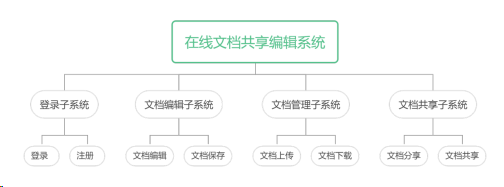
\includegraphics[height=0.2\textheight]{pic1.png}
	\caption{在线文档共享编辑系统功能结构}
	\label{fig:1}
\end{figure}

\section{登录子系统的功能}

登录子系统为程序提供了用户认证的功能,如图\ref{fig:2}所示。该系统主要实现了用户登录和注册的功能。

\begin{figure}[ht]
	\centering
	\begin{minipage}[t]{0.45\linewidth}
		\centering
		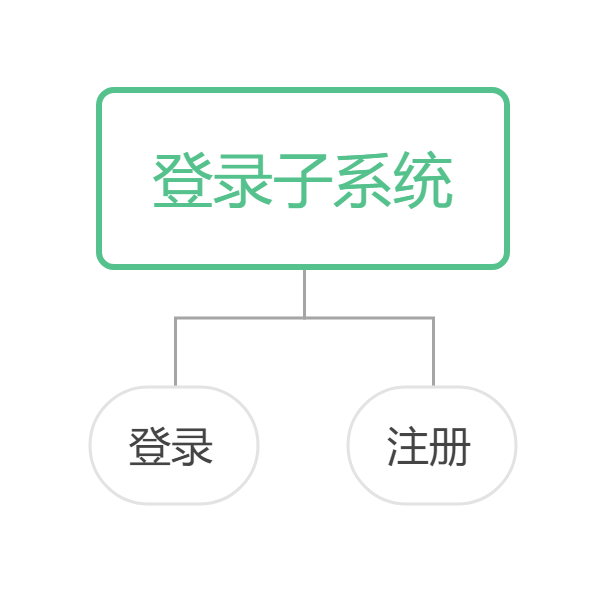
\includegraphics[height=0.2\textheight]{pic2.png}
		\caption{登录子系统功能}
		\label{fig:2}
	\end{minipage}%
	\begin{minipage}[t]{0.45\linewidth}
		\centering
		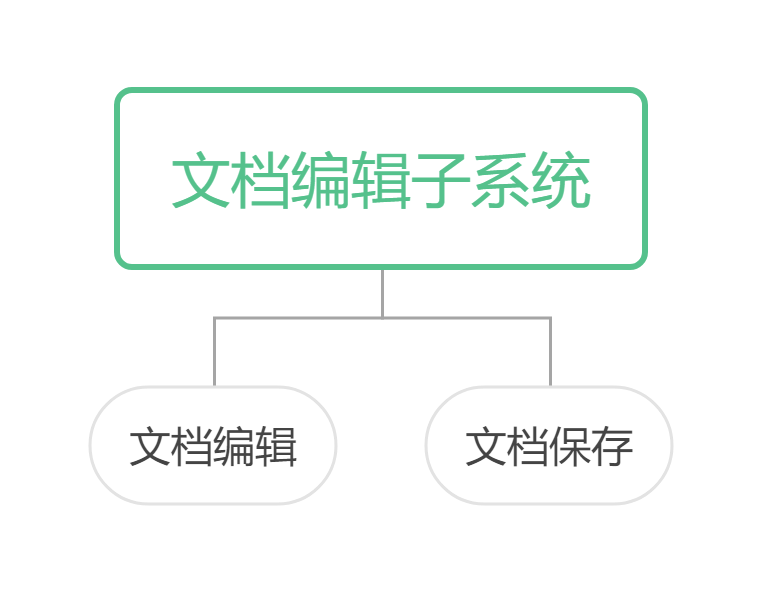
\includegraphics[height=0.2\textheight]{pic3.png}
		\caption{文档编辑子系统}
		\label{fig:3}
	\end{minipage}%
\end{figure}

\section{文档编辑子系统的功能}

文档编辑子系统提供用户编辑和保存的功能,如图\ref{fig:3}所示。用户选择需要修改的文档以后,就会弹出文本编辑框,修改完需要修改的文本时,点击保存按钮,就会把用户写的文本传输到后端文档管理服务器。

文档编辑系统的出现离不开信息技术的发展和升级换代,对于一些大企业而言,内部拥有其自建的文档编辑系统,以完成OA审批、文件传达等作用。文档编辑系统主要用于各部门之间文档互助、修改,减少因为某个单项的错误重复审批修改,其主要作用是加强对审核流存档的速度,在企业管理中起到监督、调节、指导的辅助作用[7]。

由于大企业对业务流处理的熟练,导致目前市面上的文档编辑系统区分度很高,较为完善的产品覆盖很全面,而普通的产品则只覆盖了基础的功能。

\section{文档管理子系统的功能}

文档管理子系统提供用户上传(Input)和下载(Output)的功能,是程序和本地的IO流,如图\ref{fig:4}所示。用户选择下载的文件以后,点击下载按钮,即可保存到本地,同理,点击上传按钮,就可以上传到服务器。

根据前文描述的的文档管理需求分析,本系统在设计在线共享文档编辑系统的管理系统时,采用的方式主要是是通过客户端与服务器的双向连接模式。

在这种信息管理系统的应用模式中,文档管理理系统的用户和管理员可以分别在客户端和数据库完成个体目,用户无需改变数据库,管理员也无需查看用户文本,即可分别完成他们的目的。尚若用户在编辑完成以后,通过数据库端的表内容的修改和验证,这种变化可以被即时传输到使用人员的客户端[5]。

用户在主页面提交对文件的管理需求,若用户点击上传功能,则会调用MinIO的接口工具,进行上传,根据时间编码文档名,传入数据库,并且刷新用户界面,完成文档的上传。

\begin{figure}[ht]
	\centering
	\begin{minipage}[t]{0.45\linewidth}
		\centering
		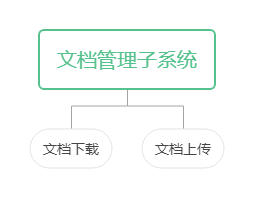
\includegraphics[height=0.2\textheight]{pic4.png}
		\caption{登录子系统功能}
		\label{fig:4}
	\end{minipage}%
	\begin{minipage}[t]{0.45\linewidth}
		\centering
		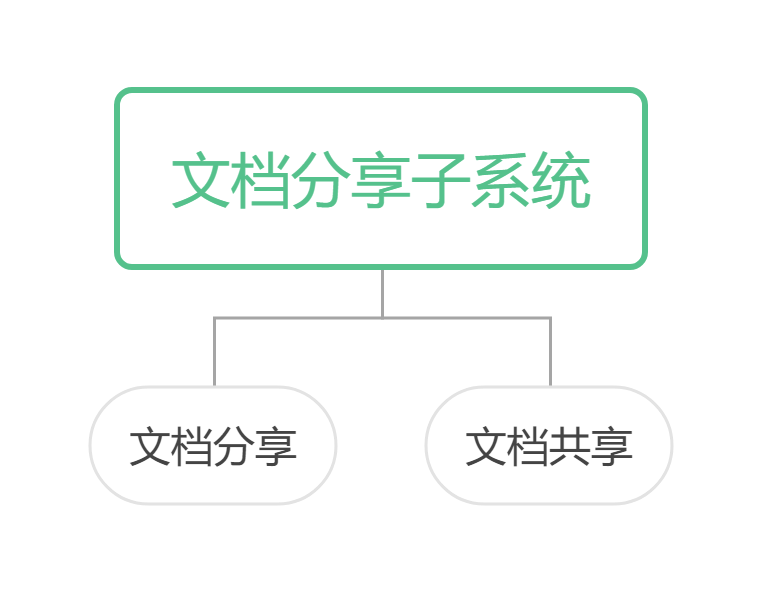
\includegraphics[height=0.2\textheight]{pic5.png}
		\caption{文档编辑子系统}
		\label{fig:5}
	\end{minipage}%
\end{figure}

对于单个用户而言,个人的用户文档数据的极易产生重复率大、数量多的缺点,尚若在某短时间不进行分拣归纳,将会导致文档拘泥,最后产生大量垃圾文件。对于文档的管理确实,就会使文档杂乱无序,不仅占用存储空间,成为稳固的垃圾文件之一,也导致用户检索其他文档产生极大地干扰,消耗大量无意义的时间做低效率的工作。真正有效的数据被淹没在大量垃圾文档中,这样的混乱降低了文档的价值表达,最终使用户厌倦对文档的处理和分发。因此,在文档编辑系统中设计一个文档管理系统尤为重要。

\section{文档分享子系统的功能}

文档共享子系统提供分享和共享的功能,是本系统设计的关键,如图\ref{fig:5}所示。用户选择文件以后,在共享id框输入域需要被共享的用户,点击共享按钮以后即可共享,可以查看和编辑;而分享则是创建一个web的html网页,将网页分享以http协议分享给其他用户,只能查看,不可编辑。

\chapter{在线编辑系统的数据库设计}

\section{本系统的数据库概念设计}

本系统数据库的概念E-R模型如图\ref{fig:6}所示,共涉及到三个表。

\begin{figure}[!htbp]
	\centering
	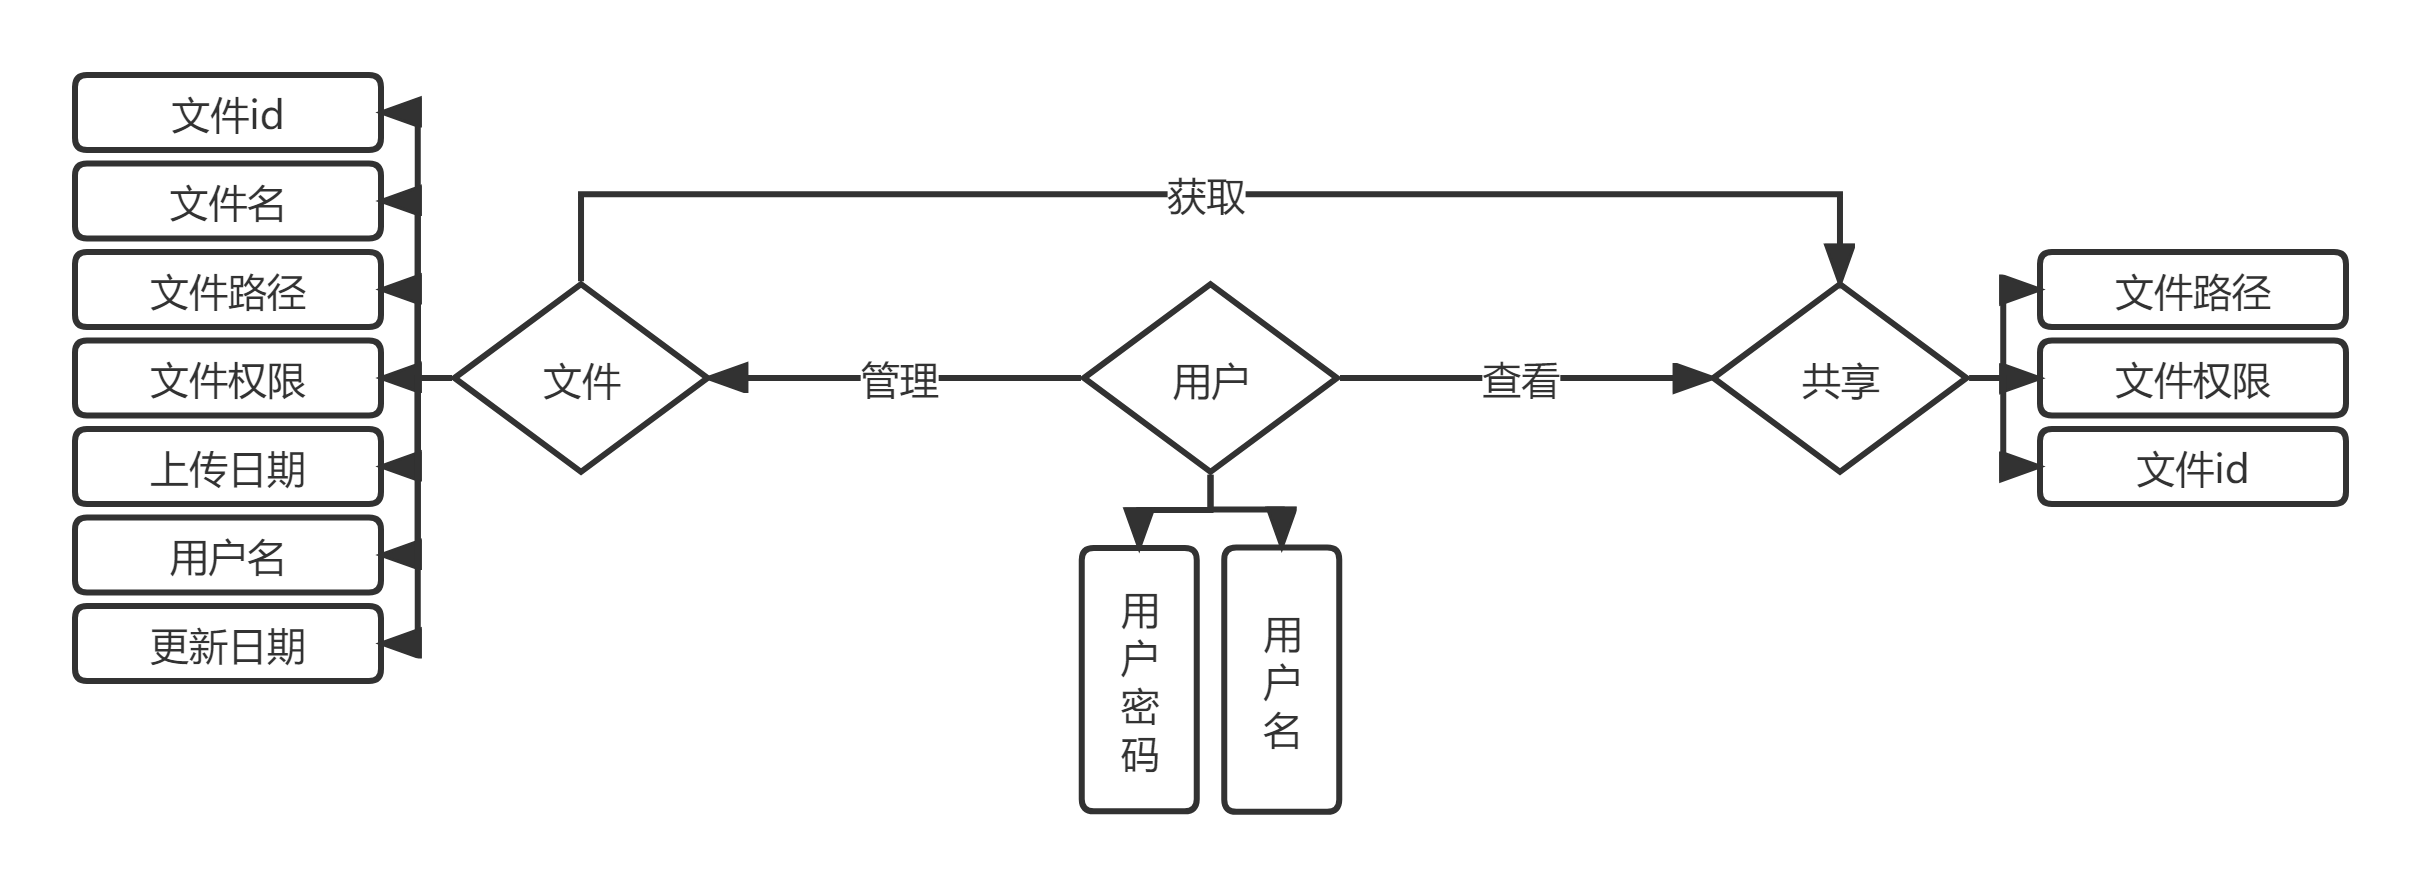
\includegraphics[height=0.2\textheight]{pic6.png}
	\caption{数据库E-R图}
	\label{fig:6}
\end{figure}

\section{本系统的数据库表设计}

本数据库如图\ref{fig:7}所示。

\begin{figure}[!htbp]
	\centering
	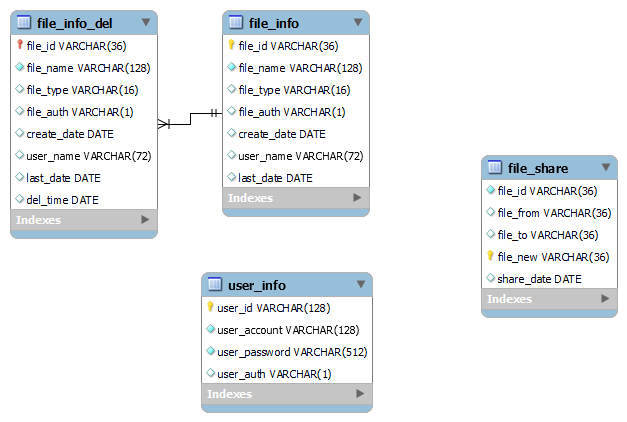
\includegraphics[height=0.2\textheight]{pic7.png}
	\caption{数据库设计图}
	\label{fig:7}
\end{figure}

file\_info和user\_info是两个基础信息表。前者记录了文件的保存信息和基础数据,使用id作为表的主键;后者记录的是用户的信息和权限,也使用id作为表的主键。

file\_share和file\_info\_del是文件分享表和文件删除表。文件分享表记录了用户分享文件的信息;文件删除表记录了用户逻辑删除的文件信息。

file\_share中,file\_new是主键,他是分享后新生成的文件信息,同时也是file\_id的外键。



\chapter{在线编辑系统的设计和实现}

本系统使用Mysql作为数据库管理系统。考虑到系统的安全性,网络环境采用星型局域网结构\upcite{r3}。

文件管理系统使用MinIO。Minio是一个高性能的负载,用作云原生应用程序的主要存储,与传统对象存储相比,云原生应用程序需要更高的吞吐量和更低的延迟。

本系统主要采用了python语言作为架构。python是一个强大的语言\upcite{r6},通过第三方的库可以对MinIO和Mysql调用。

前端使用tkinter作为界面ui,后端使用flask框架作为接口。

\section{环境配置}

本系统建立在基于linux的centos7系统下,使用pycharm对程序进行编写和测试,使用docker配置minio文件管理系统和mysql数据库管理系统。

Docker提供了一种虚拟容器技术,在目前的互联网时代被广泛使用,Docker将对象资源封装在容器内,直接使用宿主机的环境来运行镜像封装。Docker实现了虚拟机和实体机的沙箱隔离,所有的通信端口必须在用户配置镜像时预设好,虽然在一定程度上减少了程序的可调性,但是提供了更高的隔离级别,更适合用于高需求下的用户配置环境。

本项目中的minio服务端部署在服务器上,使用docker进行构建和管理。命令如下:

\begin{lstlisting}
docker search minio
docker pull minio/minio

docker run -d -p 9000:9000 -p 9090:9090 --name=minio --restart=always -e "MINIO_ROOT_USER=admin" -e "MINIO_ROOT_PASSWORD=admin123456" -v /home/data:/data -v /home/config:/root/.minio  minio/minio server /data --console-address ":9000" --address ":9090"
\end{lstlisting}

其中,`-p 9000:9000 -p 9090:9090` 表示开放端口。

--console-address ":9000" --address ":9090"

此处也需要修改为和上文一样,9000是docker容器对服务器端口,9090是管理console端口(API端口)。

--name 设置容器名字。

MINIO\_ROOT\_USER 后接管理员账号。

MINIO\_ROOT\_PASSWORD`后接管理员密码。

-v /home/data:/data -v /home/config:/root/.minio 是挂载文件的位置。

\section{本系统的总体程序控制流程}

用户在登录或者注册以后,可在平台上完成个人的文档分享和获取的需求,实现办公、交互资源的共享。通过上传或者下载,与文件进行流处理、通过分享或者共享、与其他用户协作共享。

\section{登录系统的设计和实现}

\subsection{登录系统的前端设计}

如图\ref{fig:8}所示,登录系统的交互界面包含了两个按钮:登录、注册和两个文本框:账号、密码。

\begin{figure}[!htbp]
	\centering
	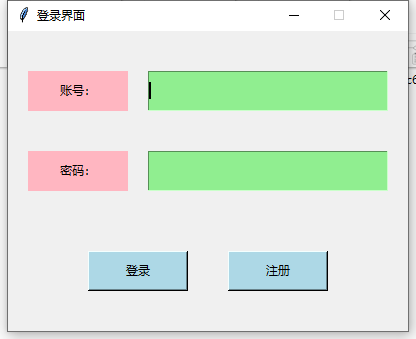
\includegraphics[height=0.2\textheight]{pic8.png}
	\caption{登录界面前端}
	\label{fig:8}
\end{figure}

登录界面实现了登录和注册两个功能。

企业在智能管理信息化系统建设的过程中应当明确内部控制目标,规范工作流程尤为重要\upcite{5}。因此,在设计密码入库的时候,需要对密码进行加密。为了确保密码的传输不以文本进行,本系统使用了md5的方法作为加密,减少因为抓包分析破解密码的可能性。

登录功能提取了用户输入的账号和密码,加密密码以后比对数据库的存档信息,如果验证成功,那么就会跳转到主界面,否则将弹出提示。

注册功能同样提取了用户输入的账号和密码,查询数据库,如果不存在该账号,提示注册成功,否则提示注册失败。

\subsection{登录系统的后端设计}

登录系统的后端定义了2个接口功能。

\begin{lstlisting}
def login(sqlClient: tool.sql.sqlClient, attrs: dict)
def register(sqlClient: tool.sql.sqlClient, attrs: dict)
\end{lstlisting}

\textbf{login接口的请求地址是:}
\begin{equation*}
	user/login
\end{equation*}

该接口可以使用POST协议接收json报文,解析为dict格式,传入参数为account和password。后端接收到数据以后,接入数据库进行搜索,如果匹配到相应的账号和密码,那么将返回用户的权限,即auth,反之,将返回code=0,前端即可知道是否应该让用户登录。

\textbf{register接口的请求地址是:}
\begin{equation*}
	user/register
\end{equation*}

该接口可以使用POST协议接收json报文,解析为dict格式,传入参数为account和password。后端接收到数据以后,接入数据库进行搜索,如果检索到账户已存在,那么将返回code=2,表示账户已存在,如果检索不到该账户,那么返回code=1,前端完成用户注册提示,后端将该用户的数据写入数据库中。

\section{文本编辑系统主界面的设计和实现}

\subsection{文本编辑系统的前端设计}

文本编辑系统的主界面用户交互设计如图\ref{fig:9}所示,左侧包括了选择文件功能,中间是文本编辑功能,右侧是文件管理系统。

\begin{figure}[!htbp]
	\centering
	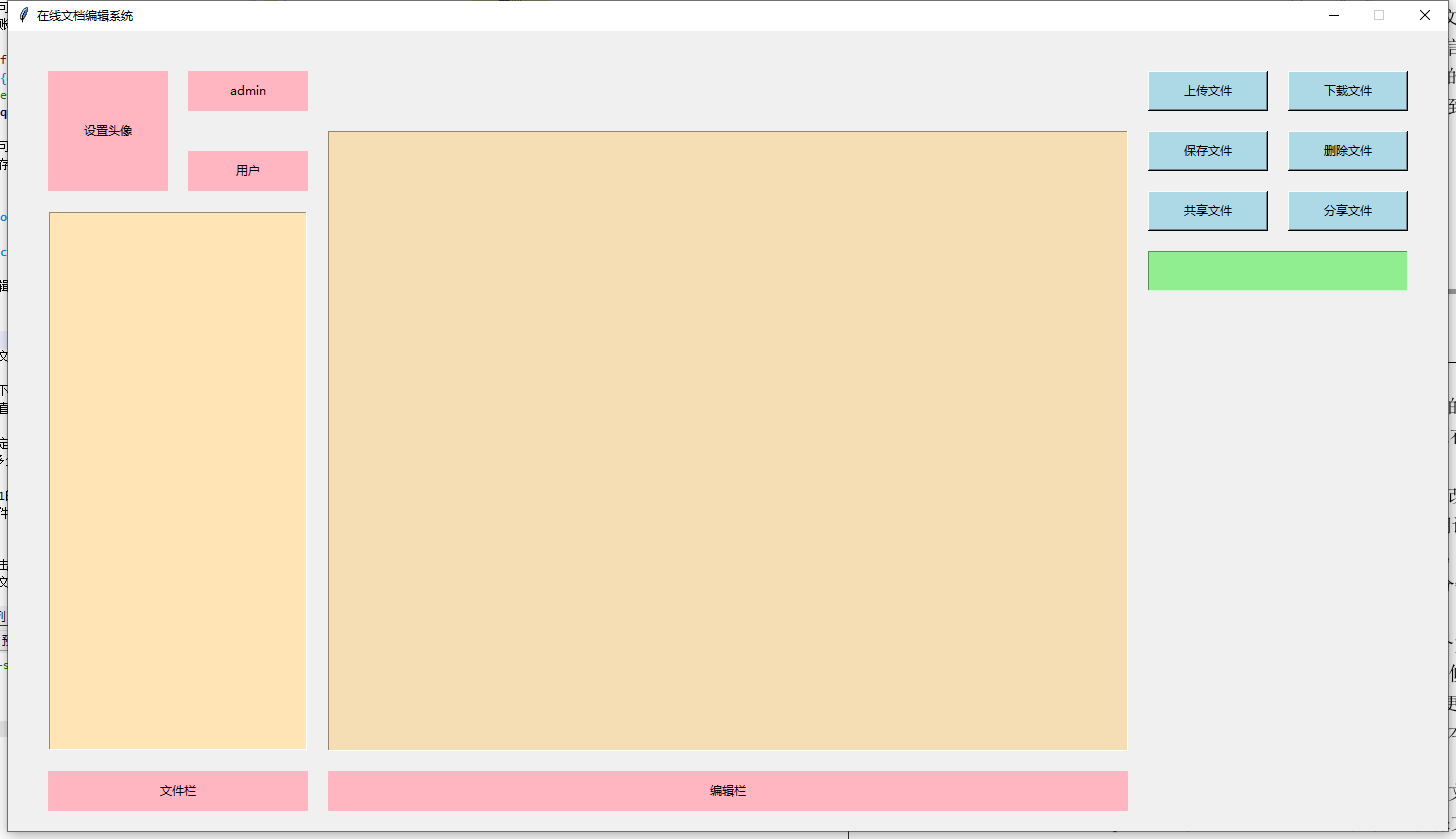
\includegraphics[height=0.2\textheight]{pic9.png}
	\caption{文本编辑系统前端}
	\label{fig:9}
\end{figure}

左侧的文件信息表为登录用户提供了文本选择的功能。用户登录以后,系统会自动查询数据库,检索用户当前存有的文件,并且显示在选择文件的框中。

用户按下任意一个文本文件的标签以后,就可以在中间文本编辑功能处的显示该文本的具体内容,如果没有提示文件正在处于其他用户编辑状态,那么用户即可直接完成对文本的编辑和修改。

文档的定位主要基于用户鼠标点击的坐标,进行计算。通过获取用户按下按钮的x,y坐标位置信息,通过公式5-1可以计算出查询文件在该用户的文件Index是多少,然后查询数据的位次,最终查询该文本的地址信息,返回该文本数据。

\begin{equation}
	Index = event.y // 20
\end{equation}

公式5-1的含义是:event.y储存了鼠标点击文件表的y轴坐标,通过对y轴坐标除以20,向下取整的方式获取到Index的值,匹配到文件表的文件id,再通过文件id去查找数据库,最终获取到文本。在python中,除以并且向下取整的符号是$//$。

用户点击文档时,首先会调用数据库,查询该文档的权限,如果权限返回值为1,那么表示可以编辑,如果返回值是0,表示有人正在编辑,用户暂时无法编辑该文档。

若用户成功打开文档以后,会向数据库发送一个修改file\_auth和last\_date值的命令,将该文本的这个值置为0,并且把最后修改日期设置为当前时间,表示文档此时处于该用户的可编辑状态,而其他用户无法访问,为了减少用户由于遗忘, 忘记关闭编辑功能导致文档长期被占用,如果用户在2分钟内不进行保存操作,那么文件权限将会释放,其他用户可以打开并编辑。

\begin{figure}[!htbp]
	\centering
	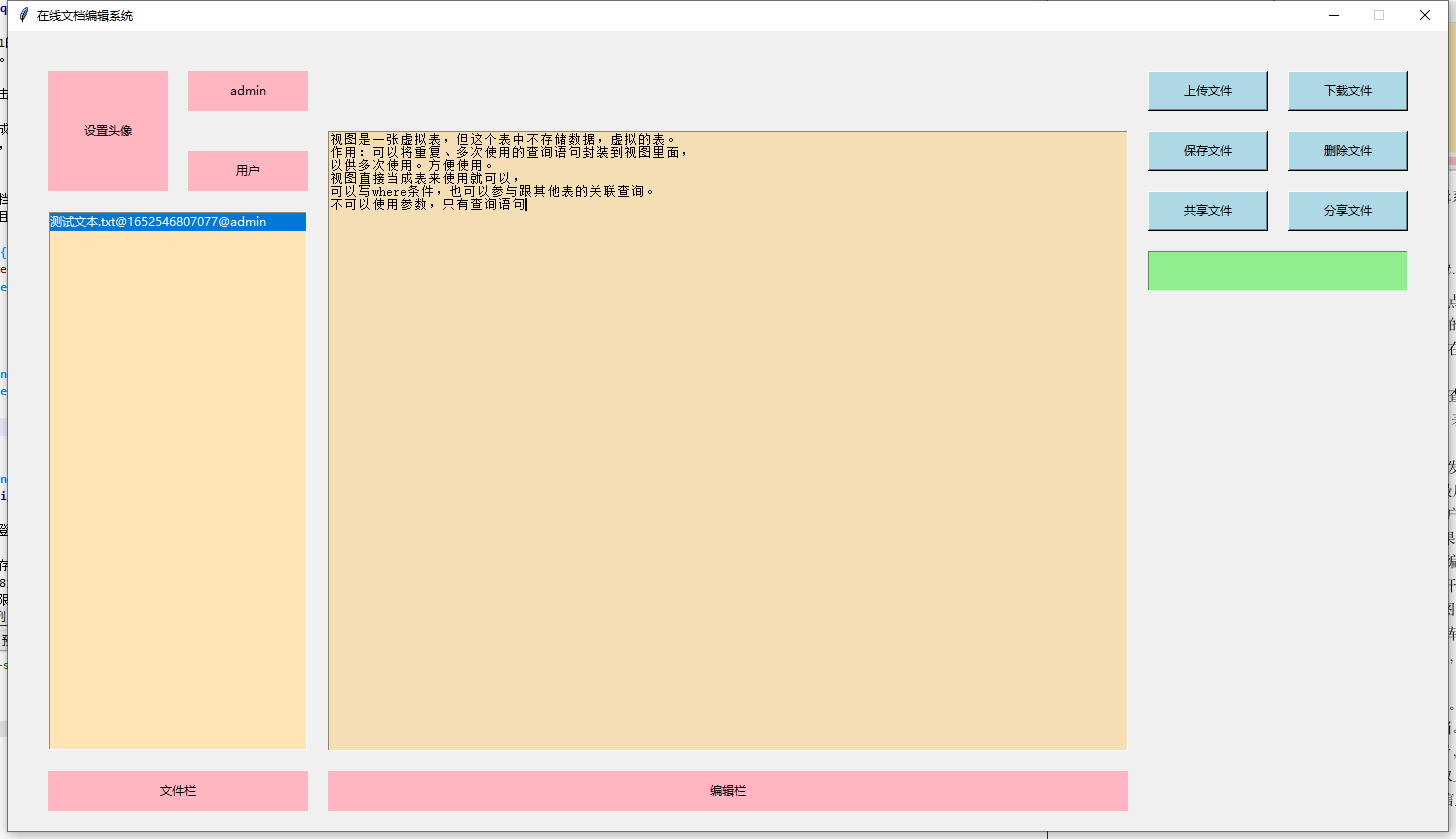
\includegraphics[height=0.15\textheight]{pic10.png}
	\caption{读取文本信息}
	\label{fig:10}
\end{figure}

编辑文档是本系统最重要的功能。以打开测试文本这个文件为例,文本编辑框显示如图\ref{fig:10},随意修改一些文本以后,这时候,点击保存按钮将最新的文本上传到文件管理服务器,并且将数据库中的最新更新日期更新到当前时间,数据库的数据如图\ref{fig:11}所示。

\begin{figure}[!htbp]
	\centering
	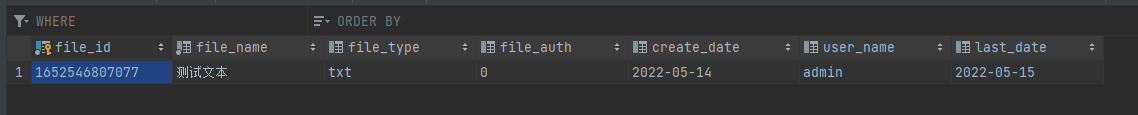
\includegraphics[height=0.05\textheight]{pic11.png}
	\caption{数据库信息}
	\label{fig:11}
\end{figure}

这时,登录另一个被共享该文档的账号,打开改文本,即可显示文档内容被成功修改为如图\ref{fig:10}的值。

文本保存的方法是对文本二进制的读写。首先读取文本编辑器的内容,在本地创建一个temp的文件,将文本写入该文档。为了确保文件解码的统一性,避免程序出错,文本的保存和读取都以utf-8进行,确保中文文本可以被成功解码。在文件写入缓存以后,调用minio的接口,获取上传链接,将二进制的文本数据使用http协议的put方法上传,最后更新数据库信息,把文件编辑权限置为1,最后更新日期传入当前时间节点。

\subsection{文本编辑系统的后端设计}

文本编辑系统的后端定义了1个接口功能。

\begin{lstlisting}
def update(minioClient: tool.mio.minioClient, mysqlClient: tool.sql.sqlClient, attrs: dict)
\end{lstlisting}

\textbf{update接口的请求地址是:}
\begin{equation*}
	file/update
\end{equation*}

使用POST协议接收json报文,解析为dict格式,传入参数为文件id。后端接收到数据以后,调用minio获取上传url地址,并且更新最新的数据库。前端接收到上传文件地址时,将文本编译为二进制流,使用PUT方法传入minio中。


\section{文档共享的设计和实现}

\subsection{文本共享的设计}

文档共享的功能是将用户A的某个文档a共享给用户B,共享成功后用户B的文档列表中也会出现文档a。

在线文档的编辑离不开对文档的管理。用户可以对文档进行上传和下载的文件管理操作。

文件的上传使用的是http协议,首先让用户对需要上传的文档进行选择,去除后缀部分的文本信息,只保留纯文件名。通过调用minio的上传接口,将文本读取为二进制的字节位,使用http协议的put方法上传文档,在文档上传成功以后,接入数据库,传入文件名、文件序号、文件权限、文件上传日期、文件来源、上传用户、最后编辑时间信息,完成对文档的入库操作。

用户也可以自行下载自己上传、修改、被共享的文档。与上传类似,文档的上传和下载主要基于http协议,通过python封装好的http协议调用,可以方便的使用minio的功能,用户首先选择一个保存目录,由于用户在打开文档时已经检查过对于该文档的权限,所以无需在此检查用户的权限。通过调用minio的下载接口,使用http协议的get方法获取文件信息,将文件保存在本地目录中。

\subsection{文本共享的后端设计}

文本共享的后端定义了3个接口功能。

\begin{lstlisting}
def upload(minioClient: tool.mio.minioClient, mysqlClient: tool.sql.sqlClient, attrs: dict)
def download(minioClient: tool.mio.minioClient, mysqlClient: tool.sql.sqlClient, attrs: dict)
def share(minioClient: tool.mio.minioClient, mysqlClient: tool.sql.sqlClient, attrs: dict)
\end{lstlisting}

\textbf{upload接口的请求地址是:}
\begin{equation*}
	file/upload
\end{equation*}

upload方法通过调用minio服务器,返回一个上传接口,使用put方法上传文件二进制流。

\textbf{download接口的请求地址是:}
\begin{equation*}
	file/download
\end{equation*}

download方法通过调用minio服务器,返回一个下载接口,使用get方法获取文件二进制流,保存到指定位置。

\textbf{share接口的请求地址是:}
\begin{equation*}
	file/share
\end{equation*}

share方法通过调用数据库,复制一份源文件,设置为新用户的一分新增文件。

\section{文档分享的设计和实现}

文档分享的功能是将用户A的某个文档a分享在互联网上。其他包括未使用该系统的用户点击这个链接,就可以直接跳转到网页上浏览这个文本的所有内容,但是不能对文本进行修改,即只有只读权限。

\begin{figure}[!htbp]
	\centering
	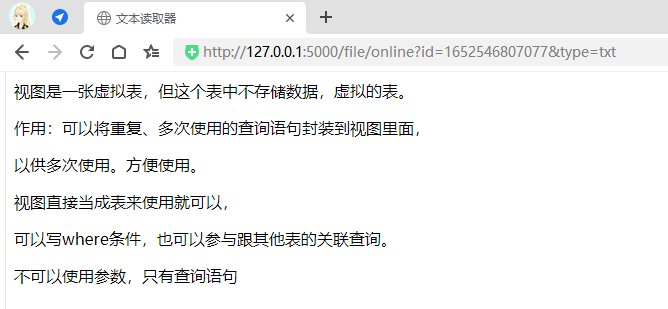
\includegraphics[height=0.2\textheight]{pic12.png}
	\caption{web前端解析文本信息}
	\label{fig:12}
\end{figure}

文档分享功能也是在线文档共享编辑系统不可缺少的一部分。用户在上传或者完成编辑以后,可以自行选择对文件进行共享和分享,如图\ref{fig:12}所示,文本被展示在浏览器上。

文档分享功能的实现主要基于flask协议传输html文本,将文档内容编码为html格式,网页最终将其渲染为文本,展示给被分享者。

文本共享是基于客户端内的编辑和使用,只能分享给使用客户端的用户。用户输入需要被共享的对象以后,客户端发送数据对数据库进行检索,如果被分享用户是自己,那么弹出提示,如果成功共享,那么会给数据库发送一个增加用户访问的指令,无异常则提示共享成功。

对于图片等非文本文件,将显示一个下载链接提供下载,如图\ref{fig:13}所示。

\begin{figure}[!htbp]
	\centering
	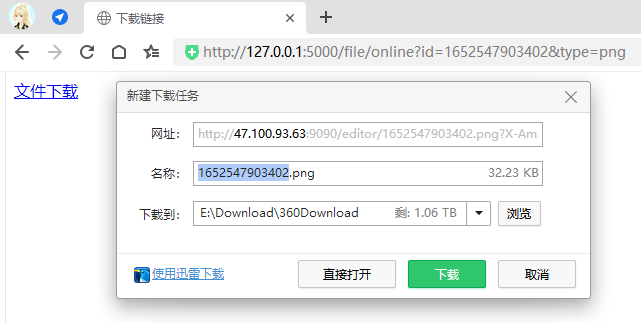
\includegraphics[height=0.2\textheight]{pic13.png}
	\caption{web前端解析非文本信息}
	\label{fig:13}
\end{figure}

\chapter{结语}

本系统在经过前期的项目调研后,成功完成对程序的需求调研和技术逻辑整理,选择了一种较为创新的在线文档底层逻辑,规划出以登录、文本共享、文本编辑和文档管理为主的四个功能结构,逐一击破,设计和实现各个需求任务。

经过数据库、程序接口、可视化界面三方面的测试,项目性能鲁棒性强,数据库冗余性高;界面功能多。

考虑不到文档共享和编辑必须建立在安全、可靠、快速的基础上。在设计开发文档共享系统,使用加密方法保存了密码信息,确保信息安全,即必须要掌握对信息可靠性的把控,权限的把握尤为关键。安全是文档编辑的基础要求,电子数据在网络上非常容易被复制和传播,必须要对非共享人员设计一个保密级别高的权限,减少人为的数据反编译产生的损失。

综上所述,本系统融合了互联网发展下的数据时代,对文档编辑系统展开研究和设计,最终建立起一套有体系的在线文档共享编辑系统。信息化的建设是一个慢长的过程,一次次的技术突破往往带来的是新时代的风向。

文档是一种拥有社会化属性的现代化元素,它在企业中是最有效的信息交换媒介。现如今,企业员工在进行文档相关工作时主要包含频繁更新内容、团队协作共同完成、紧密联系企业工作流、随时随地的浏览编辑以及标记等特点。在线文档编辑系统为团队提供了一个能够共同编辑和浏览文档的较好的方式,它能够独立的创建文字处理、表格以及演示文档。

依照在线表格编辑系统特点以及软件工程的思想,开发了多个紧密相连的模块。对于每个功能模块,均需要完成客户端和服务器端的设计。服务器端主要实现数据统一性、完整性和准确性,客户端主要实现前端和客户的交互行为。

\clearpage
%%%=== 参考文献 ========%%%
\cleardoublepage\phantomsection
\addcontentsline{toc}{chapter}{参考文献}
\begin{thebibliography}{99}

  \bibitem{r1}罗懿倩.利用Ajax技术及XML设计网络文档管理系统的思路与方法[J].电声技术,2018,42(11):61-64.DOI:10.16311/j.audioe.2018.11.017.
  \bibitem{r2}李翔.基于B/S的高校学生收费系统设计[J].电子技术与软件工程,2019(10):179-180.
  \bibitem{r3}屈武江,霍艳飞.供热收费管理系统的设计与实现[J].工业控制计算机,2021,34(11):144-145.
  \bibitem{r4}王晓燕,傅冠凯,张敏.数字化营业厅智能管理系统设计与研究[J].数字通信世界,2021(11):50-51+61.
  \bibitem{r5}孟凡波.基于高校学生管理的信息管理系统设计与实现[J].电子技术与软件工程,2021(17):169-170.
  \bibitem{r6}Katharine Jarmul,Richard Lawson.用Python写网络爬虫(第2版)[M].北京:人民邮电出版社,2018:123.
  \bibitem{r7}周奇慧.企业信息管理系统建设与维护研究[J].信息与电脑(理论版),2021,33(04):208-210.
  
\end{thebibliography}

% !Mode:: "TeX:UTF-8"
%%%%%%%%%%%%%%%%%%%%%%%%%%%%-------致谢--------%%%%%%%%%%%%%%%%%%%%%%%%%%%%%%%%

\acknowledgement
\addcontentsline{toc}{chapter}{致谢}

首先想要感谢的是本课程设计的指导老师:金世双。第一次上我他的课,是我本科二年级上学期,那时候的我对软件设计毫无概念,经过金老师一年的细心指导,终于对于软件设计有一个初步的认识,就是因为这么点滴的初步认识开启了软件开发和程序设计。感谢金老师对我的课程设计上的教导、学习上的关心,感谢金世双老三在我课程设计选题、开题直至答辩中给予我的建议和帮助!

金老师在整个过程中他给了我很大的帮忙,在论文题目制定时,他首先肯定了我的题目大方向,让我在写作时有了具体方向。在论文提纲制定时,我的思路不是很清晰,经过老师的帮忙,让我具体写作时思路顿时清晰。在完成初稿后,老师认真查看了我的文章,指出了我存在的很多问题。在此十分感谢金老师的细心指导,才能让我顺利完成本次课程设计。









 %%%致谢
\clearpage
%%%-------------- 附录. 不需要可以删除.-----------
\appendix

\chapter{事项}

本文的报告撰写使用 LaTeX 完成。

本程序已经开源在Github,地址为:

\begin{equation*}
	https://github.com/StanleySun233/OnlineEditor
\end{equation*}

\end{document}



